\documentclass[a4paper,14pt]{extarticle}

\usepackage[utf8x]{inputenc}
\usepackage[T1,T2A]{fontenc}
\usepackage[russian]{babel}
\usepackage{hyperref}
\usepackage{indentfirst}
\usepackage{here}
\usepackage{array}
\usepackage{graphicx}
\usepackage{caption}
\usepackage{subcaption}
\usepackage{chngcntr}
\usepackage{amsmath}
\usepackage{amssymb}
\usepackage{pgfplots}
\usepackage{pgfplotstable}
\usepackage[left=2cm,right=2cm,top=2cm,bottom=2cm,bindingoffset=0cm]{geometry}
\usepackage{multicol}

\renewcommand{\le}{\ensuremath{\leqslant}}
\renewcommand{\leq}{\ensuremath{\leqslant}}
\renewcommand{\ge}{\ensuremath{\geqslant}}
\renewcommand{\geq}{\ensuremath{\geqslant}}
\renewcommand{\epsilon}{\ensuremath{\varepsilon}}
\renewcommand{\phi}{\ensuremath{\varphi}}

\counterwithin{figure}{section}
\counterwithin{equation}{section}
\counterwithin{table}{section}
\newcommand{\sign}[1][5cm]{\makebox[#1]{\hrulefill}} % Поля подписи и даты
\graphicspath{{pics/}} % Путь до папки с картинками
\captionsetup{justification=centering,margin=1cm}
\def\arraystretch{1.3}

\begin{document}

\begin{titlepage}
\begin{center}
	\textbf{Санкт-Петербургский Политехнический Университет \\Петра Великого}\\[0.3cm]
	\small Институт компьютерных наук и технологий \\[0.3cm]
	\small Кафедра компьютерных систем и программных технологий\\[4cm]
	
	\textbf{ОТЧЕТ}\\ \textbf{о лабораторной работе}\\[0.5cm]
	\textbf{<<Исследование частотных характеристик пассивных RC-цепей>>}\\[0.1cm]
	\textbf{Электротехника и Электроника}\\[10.5cm]
\end{center}

\begin{flushright}
	\begin{minipage}{0.60\textwidth}
		\begin{flushleft}
			\small \textbf{Работу выполнили студенты}\\[3mm]
			\small группа 23501/4 \hspace*{17mm} Дьячков В.В.\\[3mm]
			\small группа 23501/4 \hspace*{17mm} Ламтев А.Ю.\\[5mm]
			
			\small \textbf{Преподаватель}\\[5mm]
		 	\small \sign[3.5cm] \hspace*{8mm} к.т.н., доц. Кочетков Ю.Д.\\[0.5cm]
		\end{flushleft}
	\end{minipage}
\end{flushright}

\vfill

\begin{center}
	\small Санкт-Петербург\\
	\small \the\year
\end{center}
\end{titlepage}

\section{Цель работы}

Cравнение теоретических и экспериментальных характеристик фильтров,
проектирование и настройка фильтров высокого порядка, построенных на
операционных усилителях. 

\section{Чертеж схемы исследуемого устройства}

\begin{figure}[H]
\begin{center}
	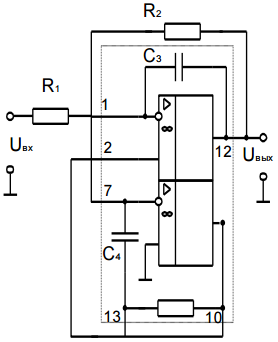
\includegraphics[width=0.4\textwidth]{scheme}
	\caption{Схема активного RC-фильтра 2 порядка}
\end{center}
\end{figure}

\section{Исходные данные}

\begin{table}[H]
\begin{center}
	\caption{Исходные данные}
	\def\tabcolsep{8pt}
	\begin{tabular}{|c|c|c|c|c|c|c|c|c|}
		\hline
		$f_{\text{м1}}$, Гц &
		$Q_1$ &
		$f_{\text{м2}}$, Гц &
		$Q_2$ &
		$\Delta L$, дБ &
		$C_3$, нФ &
		$C_4$, нФ & 
		$E_{01}$, В &
		$E_{02}$, В \\
		\hline
		500 &
		5 &
		1000 &
		5 &
		6 &
		1 &
		2 &
		15 &
		-15 \\
	    \hline	
	\end{tabular}
\end{center}
\end{table}

\section{Теоретические расчёты}

\begin{equation}
	\label{eq:4:1}
	\Delta f = \frac{f_{m, i}}{Q_i}
\end{equation}

\begin{equation}
	\label{eq:4:2}
	R_2 = (2 \pi \Delta f_i C_4)^{-1}
\end{equation}

\begin{equation}
	\label{eq:4:3}
	R_1 = \frac{C_4 R_2}{C_3 Q_i^2}
\end{equation}

\begin{equation}
	\label{eq:4:4}
	L_{m,i} = 20 lg \left( \frac{R_2 C_4}{R_1 C_3} \right)
\end{equation}

\subsection{Первое звено фильтра}

\begin{displaymath}
	\Delta f_1 = \frac{f_{m,1}}{Q_1} = \frac{500}{5} = 100 \text{ Гц}
\end{displaymath}

\begin{displaymath}
	R_2 = (2 \pi \Delta f_1 C_4)^{-1} = (2 \pi \cdot 100 \cdot 2 \cdot 10^{-9})^{-1} = 796 \text{ кОм}
\end{displaymath}

\begin{displaymath}
	R_1 = \frac{C_4 R_2}{C_3 Q_1^2} = 2 \cdot 10^{-9} \cdot 796 \cdot 10^3 \cdot \frac{1}{10^{-9} \cdot 25} = 64 \text{ кОм}
\end{displaymath}

\begin{displaymath}
	L_{m,1} = 20 lg \left( \frac{R_2 C_4}{R_1 C_3} \right) = 20 lg \left( \frac{796 \cdot 10^3 \cdot 2 \cdot 10^{-9}}{64 \cdot 10^3 \cdot 10^{-9}} \right) = 27.9
\end{displaymath}

\subsection{Второе звено фильтра}

\begin{displaymath}
	\Delta f_2 = \frac{f_{m,2}}{Q_2} = \frac{1000}{5} = 200 \text{ Гц}
\end{displaymath}

\begin{displaymath}
	R_2 = (2 \pi \Delta f_2 C_4)^{-1} = (2 \pi \cdot 200 \cdot 2 \cdot 10^{-9})^{-1} = 398 \text{ кОм}
\end{displaymath}

\begin{displaymath}
	R_1 = \frac{C_4 R_2}{C_3 Q_2^2} = 2 \cdot 10^{-9} \cdot 398 \cdot 10^3 \cdot \frac{1}{10^{-9} \cdot 25} = 32 \text{ кОм}
\end{displaymath}

\begin{displaymath}
	L_{m,2} = 20 lg \left( \frac{R_2 C_4}{R_1 C_3} \right) = 20 lg \left( \frac{398 \cdot 10^3 \cdot 2 \cdot 10^{-9}}{32 \cdot 10^3 \cdot 10^{-9}} \right) = 27.9
\end{displaymath}

\section{Экспериментально снятые зависимости}

\subsection{Первое звено фильтра}

$f_1 = 478$ Гц \\
$\delta f = 4.4 \%$ \\
$U_\text{вх} = 0.366$ В \\
$U_\text{вых} = 9.29$ В \\
$\omega_\text{рез} = 3003$ Гц \\
$L_{m1} = \frac{U_{\text{вх}}}{U_{\text{вых}}} = \frac{9.29}{0.366} = 25.4$ В \\

$U_{\text{вых}} = 9.29 \cdot 0.707 = 6.56$ В \\
$f_1^* = 436$ Гц \\
$f_2^* = 530$ Гц \\
$\Delta f^* = 94$ Гц \\
$Q = \frac{f_1}{\Delta f^*} = \frac{478}{94} = 5.08$ В \\

\begin{table}[H]
\begin{center}
	\caption{ЛАЧХ активного RC-фильтра 2 порядка}
	\label{tab:diff-int}
	\def\tabcolsep{20pt}
	\pgfplotstabletypeset[col sep=comma,
	    columns={f,u_in,u_out,k,lg_k},
	    column type/.add={|c|}{},
	    columns/f/.style={fixed, column name={$f$, Гц}},
	    columns/u_in/.style={fixed, precision=3	, zerofill, column name={$U_\text{вх}$, В}},
	    columns/u_out/.style={fixed, precision=3, zerofill, column name={$U_\text{вых}$, В}},
	    columns/k/.style={fixed, precision=3, zerofill, column name={$K$, В}},
	    columns/lg_k/.style={fixed, precision=3, zerofill, column name={$20 \cdot \lg K$, дБ}},
	    every nth row={1}{before row=\hline},
	    every head row/.style={before row=\hline, after row=\hline},
	    every last row/.style={after row=\hline}
	   ]{data/first.csv}
\end{center}
\end{table}

\begin{figure}[H]
\begin{center}
	\begin{tikzpicture} [every plot/.append style={thick}]
		\begin{axis}[
			height=0.45\textheight,
			width=0.95\textwidth,
			legend pos = north east,
			xlabel={$f$, Гц},
			ylabel={$20 \cdot \lg K$, дБ},
			axis x line = middle,
			axis y line = left,
			xmode=log,
			log basis x=2,
			xmin = 2^4,
			xmax = 2^14,
			ymin = -15,
			ymax = 35,
			grid=major
		]
		\addplot [smooth, mark=square*, blue] table[x=f,y=lg_k,col sep=comma]{data/first.csv};
		\legend{Эксп., Теор.}
		\end{axis}
	\end{tikzpicture}
	\caption{ЛАЧХ активного RC-фильтра 2 порядка}
	\label{plot:rectifier}
\end{center}
\end{figure}

\subsection{Второе звено фильтра}

$f_2 = 1000$ Гц \\
$U_\text{вх} = 0.298$ В \\
$U_\text{вых} = 9.24$ В \\
$\omega_\text{рез} = 6283$ Гц \\
$L_{m2} = \frac{U_{\text{вх}}}{U_{\text{вых}}} = \frac{9.24}{0.298} = 31$ В \\
$U_{\text{вых}} = 9.24 \cdot 0.707 = 6.53$ В \\
$f_1^* = 900$ Гц \\
$f_2^* = 1090$ Гц \\
$\Delta f^* = 190$ Гц \\
$Q_2 = \frac{f_2}{\Delta f^*} = \frac{1000}{190} = 5.26$ В \\

\begin{table}[H]
\begin{center}
	\caption{ЛАЧХ активного RC-фильтра 2 порядка}
	\label{tab:diff-int}
	\def\tabcolsep{20pt}
	\pgfplotstabletypeset[col sep=comma,
	    columns={f,u_in,u_out,k,lg_k},
	    column type/.add={|c|}{},
	    columns/f/.style={fixed, column name={$f$, Гц}},
	    columns/u_in/.style={fixed, precision=3, zerofill, column name={$U_\text{вх}$, В}},
	    columns/u_out/.style={fixed, precision=3, zerofill, column name={$U_\text{вых}$, В}},
	    columns/k/.style={fixed, precision=3, zerofill, column name={$K$, В}},
	    columns/lg_k/.style={fixed, precision=3, zerofill, column name={$20 \cdot \lg K$, дБ}},
	    every nth row={1}{before row=\hline},
	    every head row/.style={before row=\hline, after row=\hline},
	    every last row/.style={after row=\hline}
	   ]{data/second.csv}
\end{center}
\end{table}

\begin{figure}[H]
\begin{center}
	\begin{tikzpicture} [every plot/.append style={thick}]
		\begin{axis}[
			height=0.45\textheight,
			width=0.95\textwidth,
			legend pos = north east,
			xlabel={$f$, Гц},
			ylabel={$20 \cdot \lg K$, дБ},
			axis x line = middle,
			axis y line = left,
			xmode=log,
			log basis x=2,
			xmin = 2^5,
			xmax = 2^15,
			ymin = -15,
			ymax = 35,
			grid=major
		]
		\addplot [smooth, mark=square*, blue] table[x=f,y=lg_k,col sep=comma]{data/second.csv};
		\legend{Эксп., Теор.}
		\end{axis}
	\end{tikzpicture}
	\caption{ЛАЧХ активного RC-фильтра 2 порядка}
	\label{plot:rectifier}
\end{center}
\end{figure}

\subsection{Последовательно включенные звенья фильтра}

$f_{max}^1 = 490$ Гц ($U_\text{вых} = 8.9$ В) \\
$f_{max}^2 = 985$ Гц ($U_\text{вых} = 9.28$ В)\\
$f_{max}^{1,2} = 722.5$ Гц \\
$f_{min}^2 = 700$ Гц ($U_\text{вых} = 4.4$ В)\\
$U_{\text{вых}} = 9.24 \cdot 0.501 = 4.65$ В \\
$f_1^* = 432$ Гц \\
$f_2^* = 1120$ Гц \\
$\Delta f^* = 688$ Гц \\

\begin{table}[H]
\begin{center}
	\caption{ЛАЧХ активного RC-фильтра 4 порядка}
	\label{tab:diff-int}
	\def\tabcolsep{20pt}
	\pgfplotstabletypeset[col sep=comma,
	    columns={f,u_in,u_out,k,lg_k},
	    column type/.add={|c|}{},
	    columns/f/.style={fixed, column name={$f$, Гц}},
	    columns/u_in/.style={fixed, precision=3, zerofill, column name={$U_\text{вх}$, В}},
	    columns/u_out/.style={fixed, precision=3, zerofill, column name={$U_\text{вых}$, В}},
	    columns/k/.style={fixed, precision=3, zerofill, column name={$K$, В}},
	    columns/lg_k/.style={fixed, precision=3, zerofill, column name={$20 \cdot \lg K$, дБ}},
	    every nth row={1}{before row=\hline},
	    every head row/.style={before row=\hline, after row=\hline},
	    every last row/.style={after row=\hline}
	   ]{data/both.csv}
\end{center}
\end{table}

\begin{figure}[H]
\begin{center}
	\begin{tikzpicture} [every plot/.append style={thick}]
		\begin{axis}[
			height=0.45\textheight,
			width=0.95\textwidth,
			legend pos = north east,
			xlabel={$f$, Гц},
			ylabel={$20 \cdot \lg K$, дБ},
			axis x line = middle,
			axis y line = left,
			xmode=log,
			log basis x=2,
			xmin = 2^6,
			xmax = 2^13,
			ymin = 0,
			ymax = 40,
			grid=major
		]
		\addplot [smooth, mark=square*, blue] table[x=f,y=lg_k,col sep=comma]{data/both.csv};
		\legend{Эксп., Теор.}
		\end{axis}
	\end{tikzpicture}
	\caption{ЛАЧХ активного RC-фильтра 4 порядка}
	\label{plot:rectifier}
\end{center}
\end{figure}

\section{Погрешности}

\subsection{Предельно допустимые порешности}

\begin{displaymath}
\begin{aligned}
	\delta_{max} f = \delta_{max} Q = \delta_{max} L_m = \sqrt{(\delta R_1)^2 + (\delta R_2)^2 + (\delta C_3)^2 + (\delta C_4)^2} = \\ = \sqrt{0.1^2 + 0.1^2 + 0.1^2 + 0.1^2} = 0.2 = 20\%
\end{aligned}
\end{displaymath}

\begin{displaymath}
	\delta_{max} (\Delta f) = \sqrt{(\delta R_2)^2 + (\delta C_4)^2} = \sqrt{0.1^2 + 0.1^2} = 0.141 = 14.1\%
\end{displaymath}

\subsection{Приведённые погрешности}

\begin{displaymath}
	\delta f_1 = \left|\frac{f_\text{1 теор.} - f_\text{1 эксп.}}{f_\text{1 теор.}} \right| = \left|\frac{500 - 478}{500}\right| = 0.044 = 4.4\% < \delta_{max} f = 20\%
\end{displaymath}

\begin{displaymath}
	\delta f_2 = \left|\frac{f_\text{2 теор.} - f_\text{2 эксп.}}{f_\text{2 теор.}} \right| = \left|\frac{1000 - 1000}{1000}\right| = 0 = 0\% < \delta_{max} f = 20\%
\end{displaymath}

\begin{displaymath}
	\delta (\Delta f_1) = \left|\frac{\Delta f_\text{1 теор.} - \Delta f_\text{1 эксп.}}{\Delta f_\text{1 теор.}} \right| = \left|\frac{100 - 94}{100}\right| = 0.06 = 6\% < \delta_{max} (\Delta f) = 14.1\%
\end{displaymath}

\begin{displaymath}
	\delta (\Delta f_2) = \left|\frac{\Delta f_\text{2 теор.} - \Delta f_\text{2 эксп.}}{\Delta f_\text{2 теор.}} \right| = \left|\frac{200 - 190}{200}\right| = 0.05 = 5\% < \delta_{max} (\Delta f) = 14.1\%
\end{displaymath}

\begin{displaymath}
	\delta Q_1 = \left|\frac{Q_\text{1 теор.} - Q_\text{1 эксп.}}{Q_\text{1 теор.}} \right| = \left|\frac{5 - 5.08}{5}\right| = 0.016 = 1.6\% < \delta_{max} Q = 20\%
\end{displaymath}

\begin{displaymath}
	\delta Q_2 = \left|\frac{Q_\text{2 теор.} - Q_\text{2 эксп.}}{Q_\text{2 теор.}} \right| = \left|\frac{5 - 5.26}{5}\right| = 0.052 = 5.2\% < \delta_{max} Q = 20\%
\end{displaymath}

\begin{displaymath}
	\delta L_{m1} = \left|\frac{L_\text{m1 теор.} - L_\text{m1 эксп.}}{L_\text{m1 теор.}} \right| = \left|\frac{27.9 - 24.9}{27.9}\right| = 0.107 = 10.7\% < \delta_{max} L_m = 20\%
\end{displaymath}

\begin{displaymath}
	\delta L_{m2} = \left|\frac{L_\text{m2 теор.} - L_\text{m2 эксп.}}{L_\text{m2 теор.}} \right| = \left|\frac{27.9 - 31}{27.9}\right| = 0.111 = 11.1\% < \delta_{max} L_m = 20\%
\end{displaymath}

\section{Выводы}

Приведённые погрешности полученных в ходе эксперимента значений $f$, $\Delta f$, $Q$ и $L_m$ не превышают предельно допустимые погрешности.

Таким образом, формулы \ref{eq:4:1} -- \ref{eq:4:4} являются верными.

\end{document}